% Copyright (c) 2021 Eclipse Arrowhead Project
%
% This program and the accompanying materials are made available under the
% terms of the Eclipse Public License 2.0 which is available at
% http://www.eclipse.org/legal/epl-2.0.
%
% SPDX-License-Identifier: EPL-2.0

We expect the \GlossaryHyperRef{system-automation}{automation systems} of today to keep becoming more and more computerized, digitized and interconnected.
By this we mean that more aspects of and surrounding automation machines will be handled by computers, more information will be made available to those computers and, finally, comparatively more such computers will be given the opportunity to collect, communicate and act on that information.
Manufacturing, transportation, energy distribution, medicine, recycling, as well as all other industrial sectors concerned with \GlossaryHyperRef{automation}{automation} will be affected by this development.
It will lead to increased automation efficiency and flexibility, as machines become able to perform more of the work traditionally assigned to humans.
However, it will also lead to new magnitudes of complexity, not the least because of the renewed incentive to use more and more of these highly communicative machines.

The \GlossaryHyperRef{framework-arrowhead}{\textit{Arrowhead framework}} is designed to address this explosion of complexity.
It provides a foundation for \GlossaryHyperRef{communication-service-oriented}{\textit{service-oriented communication}} \cite{mackenzie2006reference} between automation systems and other computers, such that interoperability, security, safety, performance, and other major concerns can be addressed efficiently and effectively.
It notably allows for \GlossaryHyperRef{system}{system} \GlossaryHyperRef{capability}{capabilities} to be \GlossaryHyperRef{description}{described}, shared and exploited dynamically by \GlossaryHyperRef{communication}{communicating} \GlossaryHyperRef{device}{devices}.

In this document, we, the \GlossaryHyperRef{project-eclipse-arrowhead}{Eclipse Arrowhead project}, present an authoritative set of concept definitions, meant to serve as the fundamental language for describing \GlossaryHyperRef{arrowhead}{Arrowhead}-based system \GlossaryHyperRef{design}{designs}.
It exist to help mitigate compatibility and consistency issues in \GlossaryHyperRef{software}{software}, tooling, \GlossaryHyperRef{model}{models}, documentation and all other things of relevance to the Arrowhead framework.

\subsection{Primary Audiences}
\label{sec:introduction:audiences}

This document is being written and maintained for all who need precise and rigorous definitions of important \GlossaryHyperRef{arrowhead}{Arrowhead} concepts, which we understand to likely include the following groups:

\begin{itemize}
\item Advanced \GlossaryHyperRef{user}{users} of Arrowhead \GlossaryHyperRef{system}{systems}.
\item \GlossaryHyperRef{architect}{Architects} contributing to or extending the \GlossaryHyperRef{framework-arrowhead}{Arrowhead framework}.
\item \GlossaryHyperRef{developer}{Developers} of Arrowhead systems, or of devices that are expected to host Arrowhead systems.
\item \GlossaryHyperRef{operator}{Operators} of Arrowhead systems.
\item \GlossaryHyperRef{researcher}{Researchers} concerned with analyzing or refining the Arrowhead framework or Arrowhead systems.
\end{itemize}

\subsection{Scope}
\label{sec:introduction:scope}

This document is intended to clearly define all technical concepts of fundamental importance to the \GlossaryHyperRef{framework-arrowhead}{Arrowhead framework}.
It does not specify how \GlossaryHyperRef{arrowhead}{Arrowhead}-based \GlossaryHyperRef{system-automation}{automation systems} ought to be \GlossaryHyperRef{design}{designed}.
This makes its purpose analogous to that of a dictionary.
Dictionaries define words.
They may give examples of how certain words may be used, but they do not require that those words be used for any particular purposes.
This document provides an Arrowhead vocabulary other documents or models may use to express software-centric automation system designs.
It does not recommend any particular methodologies or technologies.

The concepts presented here are meant to be useful as a resource for advanced Arrowhead framework learners, as well as to serve as foundation for other documentation and modeling efforts.
This document does \textit{not} define an Arrowhead profile for SysML \cite{omg2019sysml}, or any other modeling language.
For those interested in using this document for software-architectural purposes, a description of how it can be used as a \GlossaryHyperRef{metamodel}{metamodel} in the context of an ISO/IEC/IEEE 42010 \GlossaryHyperRef{kind-model}{model kind} is provided in Section \ref{sec:conformance:iso42010}.

\newpage

\subsection{Notational Conventions}
\label{sec:introduction:conventions}

This document adheres to the notational conventions presented in the below subsections.

\subsubsection{Graph Diagrams}
\label{sec:introduction:conventions:graphs}

In a graph diagram, a box with a solid border and a name inside it denotes a named model \GlossaryHyperRef{entity}{entity}, representing an \GlossaryHyperRef{artifact}{artifact} or \GlossaryHyperRef{stakeholder}{stakeholder}.
Model entities can be associated with \GlossaryHyperRef{attribute}{attributes} by describing those attributes in text in relation to the diagrams in which they occur.
A named arrow from a source box to a target box denotes the \GlossaryHyperRef{relationship}{relationship} implied by the name.
Relationship names are defined either here, in the glossary of Section \ref{sec:glossary}, or in relation to the figures they are used in.
The following relationship names are defined here only:

\begin{enumerate}
\item \textit{conforms to}, implying that the target \textit{has} a set of \GlossaryHyperRef{constraint}{constraints} satisfied by the source;
\item \textit{extends}, meaning that the source \textit{conforms to} and inherits all relationships and attributes of the target;
\item \textit{is}, meaning that the source \textit{extends} the target and belongs to a set named after it;
\item \textit{uses}, meaning that the source depends on the target to fulfill its purpose;
\item \textit{has}, meaning that the target is \textit{used by} and must cease to exist without the source; and
\end{enumerate}

\paragraph{Quantifiers}
If an arrow has an associated positive integer or range, which we refer to as a \textit{quantifier}, the relationship is to be considered as extending to the number of distinct entities indicated by that quantifier.
No quantifier being associated with a certain relationship implies that it has a quantity of 1.
A range is denoted by $x..y$, where $x$ and $y$ are integers and $0 \leq x < y$.
If $y$ is substituted by $*$, the range is to be understood to extend infinitely from $x$ (e.g. ``$1..*$'').

\paragraph{Grouped Relationships}
To save space or improve clarity, arrows are sometimes grouped such that either their target or source ends are shared, as in Figure \ref{fig:graph-diagram}.
If such a group of arrows has a relationship name closest to its shared part, it must be understood to apply to each arrow of the group, as if they were not grouped at all.
Relationship quantifiers are always closest to the non-shared parts.
Grouped arrows can always be replaced with non-grouped arrows without loss of information.

\vfill

\begin{figure}[ht!]
  \centering
  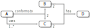
\includegraphics[scale=0.9]{figures/graph-diagram}
  \caption{
    An example graph diagram.
    \textbf{A} \textit{conforms to} 1 \textbf{B}, as no quantifier is associated with the arrow from \textbf{A} to \textbf{B} and 1 is the default quantity.
    \textbf{A} also \textit{conforms to} 2 \textbf{C}s, as well as \textit{uses} 1 or more \textbf{C}s.
    Both \textbf{B} and \textbf{C} \textit{has} 2 \textbf{D}s.
  }
  \label{fig:graph-diagram}
\end{figure}

\subsubsection{References}

Square brackets around integers (e.g. \cite{delsing2017iot}) are references to the reference list in Section \ref{sec:references}.
The integer within the brackets of any given reference corresponds to the entry with the same integer in the reference list.

References within this document are hyperlinked, which means that those reading it electronically can click the references and immediately be taken to their targets.
Special treatment is given to references targeting Section \ref{sec:glossary}, the \nameref{sec:glossary}.
These are displayed as regular text rendered with blue color.

\subsubsection{Requirements}

Use of the terms \textbf{must}, \textbf{must not}, \textbf{should}, \textbf{should not} and \textbf{may} are to be interpreted as follows when used in this document: \textbf{must} and \textbf{must not} denote absolute requirements and prohibitions, respectively; \textbf{should} and \textbf{should not} denote recommendations that should be deviated from only if special circumstances make it relevant; and, finally, \textbf{may} denotes something being truly optional.

\newpage

\subsection{Relationships to Other Documents}
\label{sec:introduction:relationships}

This document reuses or builds upon the concepts presented in the following works:

\begin{enumerate}

\item \textbf{IoT Automation: Arrowhead Framework} (IoTA:AF) \cite{delsing2017iot}, which significantly includes an overview of the \GlossaryHyperRef{cloud-local-automation}{\textit{local automation cloud}} concept in its second chapter, as well as the \textit{\GlossaryHyperRef{framework-arrowhead}{Arrowhead framework} \GlossaryHyperRef{architecture}{architecture}} in its third chapter.
The book most significantly represents the state of the Arrowhead framework up until it was written.
Even though the \GlossaryHyperRef{framework}{framework} has evolved since then, it still represents the most comprehensive description of the framework.
While the strictly architectural aspects of IoTA:AF are outside the scope of this document, the two mentioned chapters contain several definition with a high degree of relevance here.

\item \textbf{ISO/IEC/IEEE 42010 Systems and software engineering — Architecture description} (ISO42010) \cite{iso42010}, which outlines a standardized approach to structuring architectural documents and \GlossaryHyperRef{model}{models}.
The standard is adhered to in the sense that the definitions of this document are meant to be useful as a metamodel part of a so-called \GlossaryHyperRef{kind-model}{\textit{model kind}}, as defined by the standard.
No claim of conformance to the standard is made for this document on its own.
Please refer to Section \ref{sec:conformance:iso42010} for more details.

\item \textbf{Reference Model for Service Oriented Architecture} (SOA-RM) \cite{mackenzie2006reference}, which provides a standardized definition of Service-Oriented Architecture (SOA).
\GlossaryHyperRef{communication}{Communications} between \GlossaryHyperRef{arrowhead}{Arrowhead} \GlossaryHyperRef{system}{systems} are expected to adhere to this paradigm, which is what makes the standard relevant here.

\item \textbf{Reference Architecture Model Industrie 4.0} (RAMI4.0) \cite{adolphs2016reference}, which outlines an ontological and architectural description of \GlossaryHyperRef{industry40}{\textit{Industry 4.0}}.
The document may be seen as a predecessor to, or major influence on, the conceptual aspects of the Arrowhead framework.
In particular, the document describes how to model and design communicating industrial systems such that key Industry 4.0 characteristics can be facilitated, such as high degrees of dynamicity and interoperability.
However, as RAMI4.0 is a reference \textit{architecture} rather than a reference \textit{model}, we have only been concerned with what concepts it defines and what problems it frames.
This delimitation excludes its ``architectural layers'', ``life-cycle \& value-stream'' phases and ``hierarchical levels'', as well as the abstract design of its ``asset administrative shell''.
These excluded aspects are neither condemned nor endorsed by this document.
They are simply outside its scope.

\end{enumerate}

Only conformity with IoTA:AF and ISO42010 is observed strictly, which means that concept definitions presented here may diverge from those of the other two works.
All significant terminology differences are noted in the glossary of Section \ref{sec:glossary}, which provides a brief definition of each concept of relevance to this document.

\subsection{Section Overview}
\label{sec:introduction:sections}

The remaining sections of this document are organized as follows:
\vspace*{2mm}
\begin{itemize}[leftmargin=2cm,rightmargin=0pt,labelwidth=2cm,labelsep=0pt,itemindent=0pt,parsep=0.1cm,topsep=0.1cm,align=left]

\item[Section \ref{sec:introduction}]
This section.

\item[Section \ref{sec:overview}]
A brief and formal overview of \GlossaryHyperRef{arrowhead}{Arrowhead}, describing how its core concepts relate to each other.
The section also serves to provide a workable summary of the \GlossaryHyperRef{framework}{framework} and to prepare readers for better understanding Section \ref{sec:concepts}.

\item[Section \ref{sec:concepts}]
A formal description of the most significant concepts of Arrowhead.
Each of its subsections is concerned with one primary concept, ranging from \GlossaryHyperRef{entity}{entities} to \GlossaryHyperRef{system-of-local-clouds}{systems-of-local-clouds}.

\item[Section \ref{sec:conformance}]
A list of requirements, meant to help determine if a document or \GlossaryHyperRef{model}{model} referring to the concepts of this document can be considered conformant.
A special subsection on ISO/IEC/IEEE 42010 conformance is also provided.

\item[Section \ref{sec:glossary}]
Lists all significant terms and abbreviations presented in this document in alphabetical order.

\item[Section \ref{sec:references}]
Lists references to publications referred to in this document.

\item[Section \ref{sec:revision}]
Records the history of officially ratified changes made to this document.

\end{itemize}
